\newlength{\nodesep}
\setlength{\nodesep}{0.8cm} % distance between nodes
\newlength{\innersep}
\setlength{\innersep}{2pt}  % inner separation within nodes
\newlength{\sep}
\setlength{\sep}{1.1cm}    % uniform separation for both vertical and horizontal

\tikzset{
    observed/.style={circle, draw, thick, fill=gray!50, minimum size=.7cm},
    unobserved/.style={circle, draw, thick, minimum size=1.2cm},
    blank/.style={circle, draw, thick, dotted, minimum size=.7cm, opacity=0.5},
    plate/.style={draw, dotted},
    square1/.style={draw, fill=gray!20, minimum size=.3cm},
    square2/.style={draw, fill=gray!50, minimum size=.3cm},
    square3/.style={draw, fill=gray!100, minimum size=.3cm},
    true/.style = {circle, draw=none, thick, fill=green!50, minimum width=.5cm, minimum height=.5cm, inner sep=0pt},
    false/.style = {circle, draw=none, thick, fill=red!50, minimum width=.5cm, minimum height=.5cm, inner sep=0pt},
    plain/.style = {circle, draw, thick, fill=none, minimum width=.5cm, minimum height=.5cm, inner sep=0pt},
    arrowstyle/.style={->, thick, rounded corners},
    arrowstyledash/.style={->, thick, rounded corners, dash pattern=on 2pt off .6pt, gray},
    adjweight/.style={->, dashed, line width=.1mm, color=blue!50},
    adjweightbig/.style={->, line width=.6mm, color=blue!50},
    cembtrue1/.style={draw, fill=green!20, minimum size=.3cm},
    cembtrue2/.style={draw, fill=green!50, minimum size=.3cm},
    cembtrue3/.style={draw, fill=green!100, minimum size=.3cm},
    cembfalse1/.style={draw, fill=red!20, minimum size=.3cm},
    cembfalse2/.style={draw, fill=red!50, minimum size=.3cm},
    cembfalse3/.style={draw, fill=red!100, minimum size=.3cm},
    operation/.style={draw, thick, fill=blue!20, minimum size=0.6cm,  rounded corners=5pt, inner sep=1pt, outer sep=0pt, align=center},
}


\newcommand{\model}{
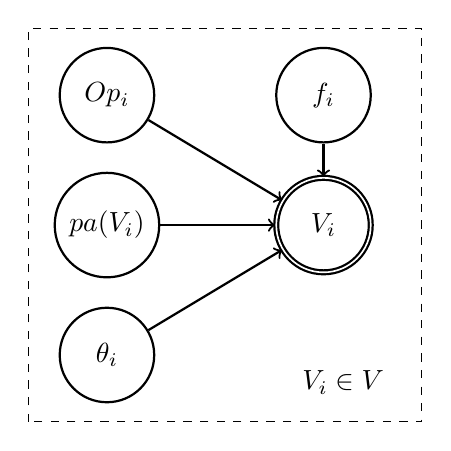
\begin{tikzpicture}[
    node distance = .3cm,
]

\node[unobserved] (var) at (0,0) {$\text{pa}(V_i)$};
\node[unobserved] (func) at (2.5*\sep,1.5*\sep) {$f_i$};
\node[unobserved] (op) at (0,1.5*\sep) {$Op_i$};
\node[unobserved] (params) at (0,-1.5*\sep) {$\theta_i$};
\node[unobserved, double] (out) at (2.5*\sep,0) {$V_i$};

\draw[arrowstyle] (var) -- (out);
\draw[arrowstyle] (op) -- (out);
\draw[arrowstyle] (params) -- (out);
\draw[arrowstyle] (func) -- (out);

\draw[dashed] (-1.,-2.5) rectangle (4., 2.5);
\node at (3., -2) {$V_i \in V$};

\end{tikzpicture}
}


\newcommand{\equivariance}{
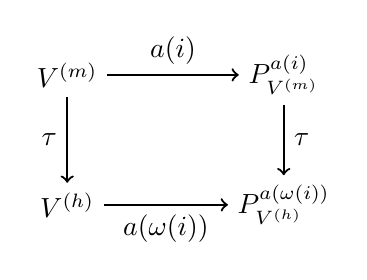
\begin{tikzpicture}[
    node distance = .3cm,
]
\node[] (intH) at (0,0) {$V^{(m)}$};
\node[] (intM) at (2.5*\sep,0) {$\mathbb{P}_{V^{(m)}}^{a(i)}$};
\node[] (PH) at (0,-1.5*\sep) {$V^{(h)}$};
\node[] (PM) at (2.5*\sep,-1.5*\sep) {$\mathbb{P}_{V^{(h)}}^{a(\omega(i))}$};

\draw[arrowstyle] (intH) -- (PH) node[midway, left] {$\tau$};
\draw[arrowstyle] (intH) -- (intM) node[midway, above] {$a(i)$};
\draw[arrowstyle] (intM) -- (PM) node[midway, right] {$\mathcal{\tau}$};
\draw[arrowstyle] (PH) -- (PM) node[midway, below] {$a(\omega(i))$};


\end{tikzpicture}
}


\newcommand{\equivarianceSurrogate}{
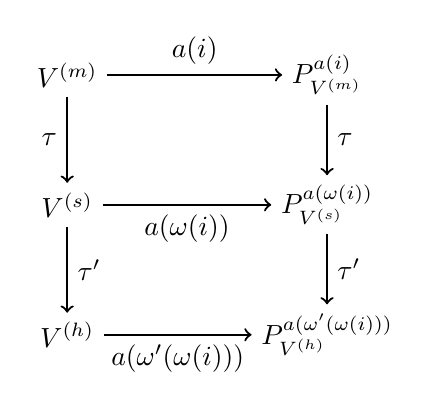
\begin{tikzpicture}[
    node distance = .3cm,
]
\node[] (intH) at (0,0) {$V^{(m)}$};
\node[] (intM) at (3*\sep,0) {$\mathbb{P}_{V^{(m)}}^{a(i)}$};
\node[] (PH) at (0,-1.5*\sep) {$V^{(s)}$};
\node[] (PM) at (3*\sep,-1.5*\sep) {$\mathbb{P}_{V^{(s)}}^{a(\omega(i))}$};
\node[] (PS) at (0,-3*\sep) {$V^{(h)}$};
\node[] (PS2) at (3*\sep,-3*\sep) {$\mathbb{P}_{V^{(h)}}^{a(\omega'(\omega(i)))}$};

\draw[arrowstyle] (intH) -- (PH) node[midway, left] {$\tau$};
\draw[arrowstyle] (intH) -- (intM) node[midway, above] {$a(i)$};
\draw[arrowstyle] (intM) -- (PM) node[midway, right] {$\tau$};
\draw[arrowstyle] (PH) -- (PM) node[midway, below] {$a(\omega(i))$};
\draw[arrowstyle] (PH) -- (PS) node[midway, right] {$\tau'$};
\draw[arrowstyle] (PM) -- (PS2) node[midway, right] {$\tau'$};
\draw[arrowstyle] (PS) -- (PS2) node[midway, below] {$a(\omega'(\omega(i)))$};


\end{tikzpicture}
}